\section{Heart model}
\label{sec:heartcellularautomata}
For the verification of \acp{ICD},
we adopt the \acf{CA}-based heart model developed in \cite{Spector11_Emergence},\cite{StinnettDonnelly12_EGMresolution}.
%Like \cite{BartocciCBESG09_HIOAmodeling}, it is based on \acf{CA} and is augmented with differential equations in each cell to describe the evolution of the transmembrane voltage with time.
This model lies in-between high spatial fidelity but slow to compute PDE-based whole heart models  \cite{vfiborganization_Tusscher07}, and low spatial fidelity but very fast-to-compute automata-based models \cite{TECS}.
PDE-based models are not currently amenable to formal verification, both theoretically and practically, and timed automata models can not simulate the electrograms needed for \ac{ICD} verification.
\ac{CA}-based models were used in \cite{Mery},\cite{BartocciCBESG09_HIOAmodeling} and \cite{Chen14_Quantitative}.
This model also has the important advantage of forming the basis of software used to train physicians and electrophysiologists, and allows interactive simulation of surgical procedures like ablation \cite{visibleep}.

In showing the various systems are STORMED, we partially depend on the specifics of the systems we model. 
The key observations are that, as will be seen in Section \ref{sec:discriminators},
i) the \ac{ICD} will always reach a decision of VT or SVT in finite time, 
ii) at which point it flushes its variables so new values are computed for the next arrhythmia episode.
So while the heart can beat indefinitely, for the purposes of \ac{ICD} verification, 
there's a uniform upper bound on the length of time of any execution.
Let $D \geq 0$ be this duration ($D$ is on the order of 30sec depending on device settings).
Moreover, the \ac{EGM} voltage signal $\egm$ has upper and lower bounds $\egm_M$ and $\egm_m$.
We also use the general results on STORMED systems that we establish in Sections  \ref{sec:compositionality}-\ref{sec:simulationAprox}.
%
%Past this time, the \ac{ICD} algorithm starts over, so we may consider that the entire system starts over.
% and may be viewed as simplifications of \cite{ChernyakFC97_PhysRevE}.
%We also use an electrode measurement model that captures the electric waveforms captured by the \ac{ICD} electrodes.
%\subsection{Basic cardiac electrophysiology}
%The heart has two upper chambers called the \emph{atria} and two lower chambers called the \emph{ventricles} (Fig. \ref{fig:icd})
%The synchronized contractions of atria and ventricles deliver an adequate supply of oxygenated blood to the rest of the body.
%This contraction is driven by electrical activity in the heart.
%Under normal conditions, the SinoAtrial (SA) node (a tissue in the right atrium) spontaneously \emph{depolarizes}, producing an electrical wave that propagates to the atria and then down to the ventricles (Fig.\ref{fig:whole heart})
%This is referred to as the \ac{NSR}.
%Disturbances of \ac{NSR} are known as \emph{arrhythmias}, and can result in insufficient blood supply and even death of a patient. 
%\emph{\ac{VT}} is an example of an arrhythmia originating in the ventricles, in which the ventricles spontaneously beat at a very high rate.
%If the \ac{VT} is sustained, or degenerates into \ac{VF}, it is fatal within seconds.
%An abnormally fast heart rate that originates in the atria is referred to as a \emph{\ac{SVT}}.
%This is a diseased but non-fatal condition, and many arrhythmias fall under this heading.
%In what follows, we will refer to sustained \ac{VT} and \ac{VF} together as \ac{VT}.
%%
\subsection{Cellular automata model}
%\begin{figure}[t]
%	\centering
%	\vspace{-10pt}
%	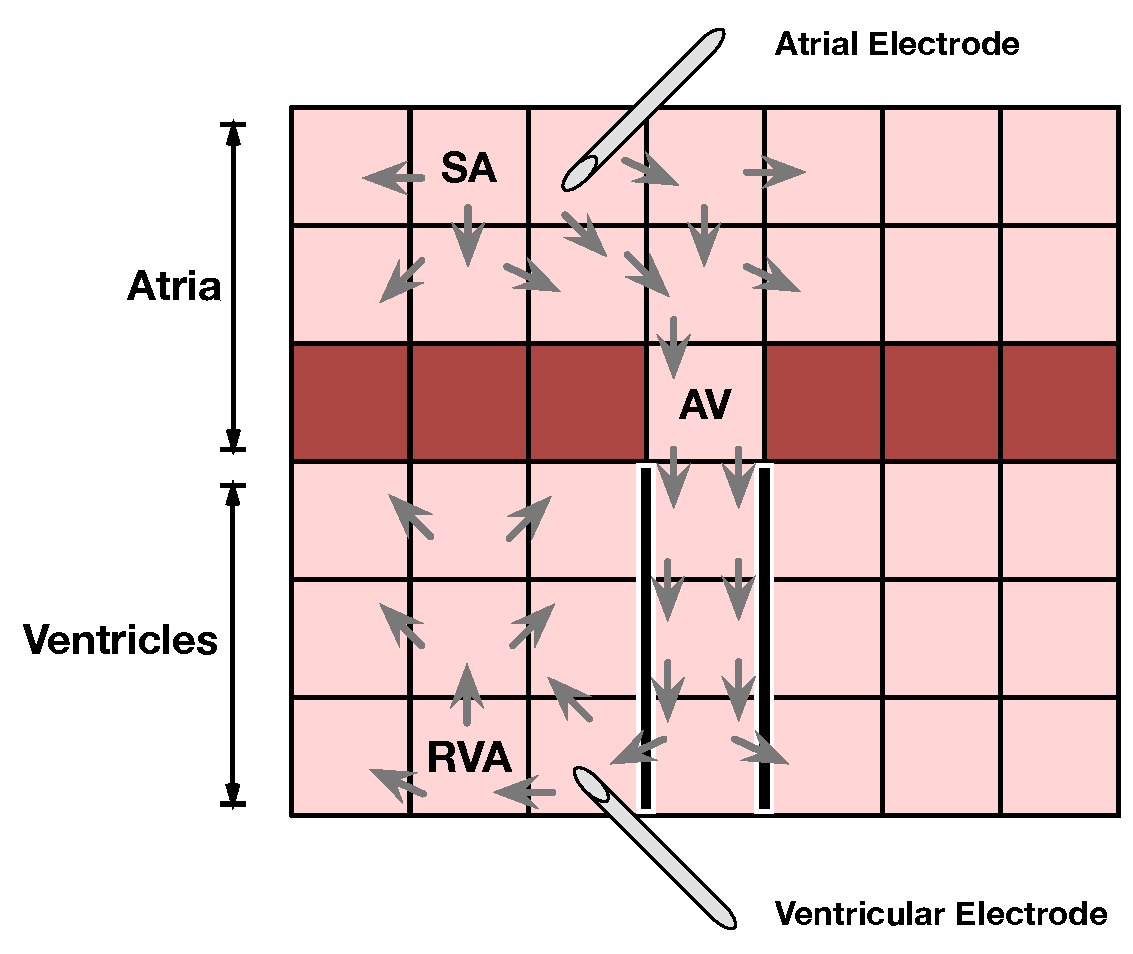
\includegraphics[scale=0.35]{figures/wholeHeartMesh}
%	\vspace{-10pt}
%	\caption{\small Whole heart modeled as a 2D mesh of cells. The \ac{ICD} leads are shown in the right atrium and ventricle. \textbf{AV}: atrio-ventricular node, \textbf{RVA}: right ventricle apex, \textbf{SA}: sino-atrial node.}
%	\label{fig:whole heart}
%	\vspace{-10pt}
%\end{figure}
The heart has two upper chambers called the \emph{atria} and two lower chambers called the \emph{ventricles} (Fig. \ref{fig:icd})
The synchronized contractions of the heart are driven by electrical activity.
Under normal conditions, the SinoAtrial (SA) node (a tissue in the right atrium) spontaneously \emph{depolarizes}, producing an electrical wave that propagates to the atria and then down to the ventricles (Fig.\ref{fig:overview})
In this model, the myocardium (heart's muscle) is treated as a 2D surface (so it has no depth), and discretized into \emph{cells}, which are simply regions of the myocardium (Fig. \ref{fig:overview}). 
Thus we end up with $N^2$ cells in a square $N$-by-$N$ grid.
A cell's voltage changes in reaction to current flow from neighboring cells, and in response to its own ion movements across the cell membrane.
This results in an \emph{\ac{AP}}.

Fig. \ref{fig:cellaut} shows how the \ac{AP} is generated by a given cell \cite{Klabunde_CVEPconcepts}:
in its quiescent mode (Phase 4), a cell $(i,j)$ in the grid has a cross-membrane voltage $V(i,j,t)$ equal to $V_{min} < 0$.
As it gathers charge, $V(i,j,t)$  increases until it exceeds a threshold voltage $V_th$.
The voltage then experiences a very fast increase, called the upstroke, to a level $V_{max} > 0$, after which it decreases to a plateau.
It stays at the plateau level for a certain amount of time \textbf{PD}  then decreases linearly to below $V_{th}$ (Phase 3 - ERP).
Once below $V_{th}$ it is said to be in the Relative Refractory Period (RRP).
In RRP, the cell can be depolarized a second time, albeit at a higher threshold $V_{th,2}$, slower and to a lower plateau level $V_{max,2} < V_{max}$.
Otherwise, when the voltage reaches $V_{min}$ again, the cell enters the quiescent stage again. 
This model is suitable for both pacemaker and non-pacemaker cells, the main differences being in the duration of the plateau (virtually non-existent for pacemaker cells), and the duration of phases 0 and 4 (both are shorter for pacemaker cells).

In Fig. \ref{fig:cellaut}, $V(i,j,t) \in \Re$ denotes the voltage in cell $(i,j)$ of the grid at time $t$, and vector $V =(V(1,1),\ldots, V(N^2,N^2))^T$ in $\Re^{N^2}$ groups the cross-membrane voltages of all cells in the heart.
The whole heart model $\Sys_{CA}$ is the parallel composition of these $N^2$ single-cell models. 
\begin{figure}[t]
	\centering
	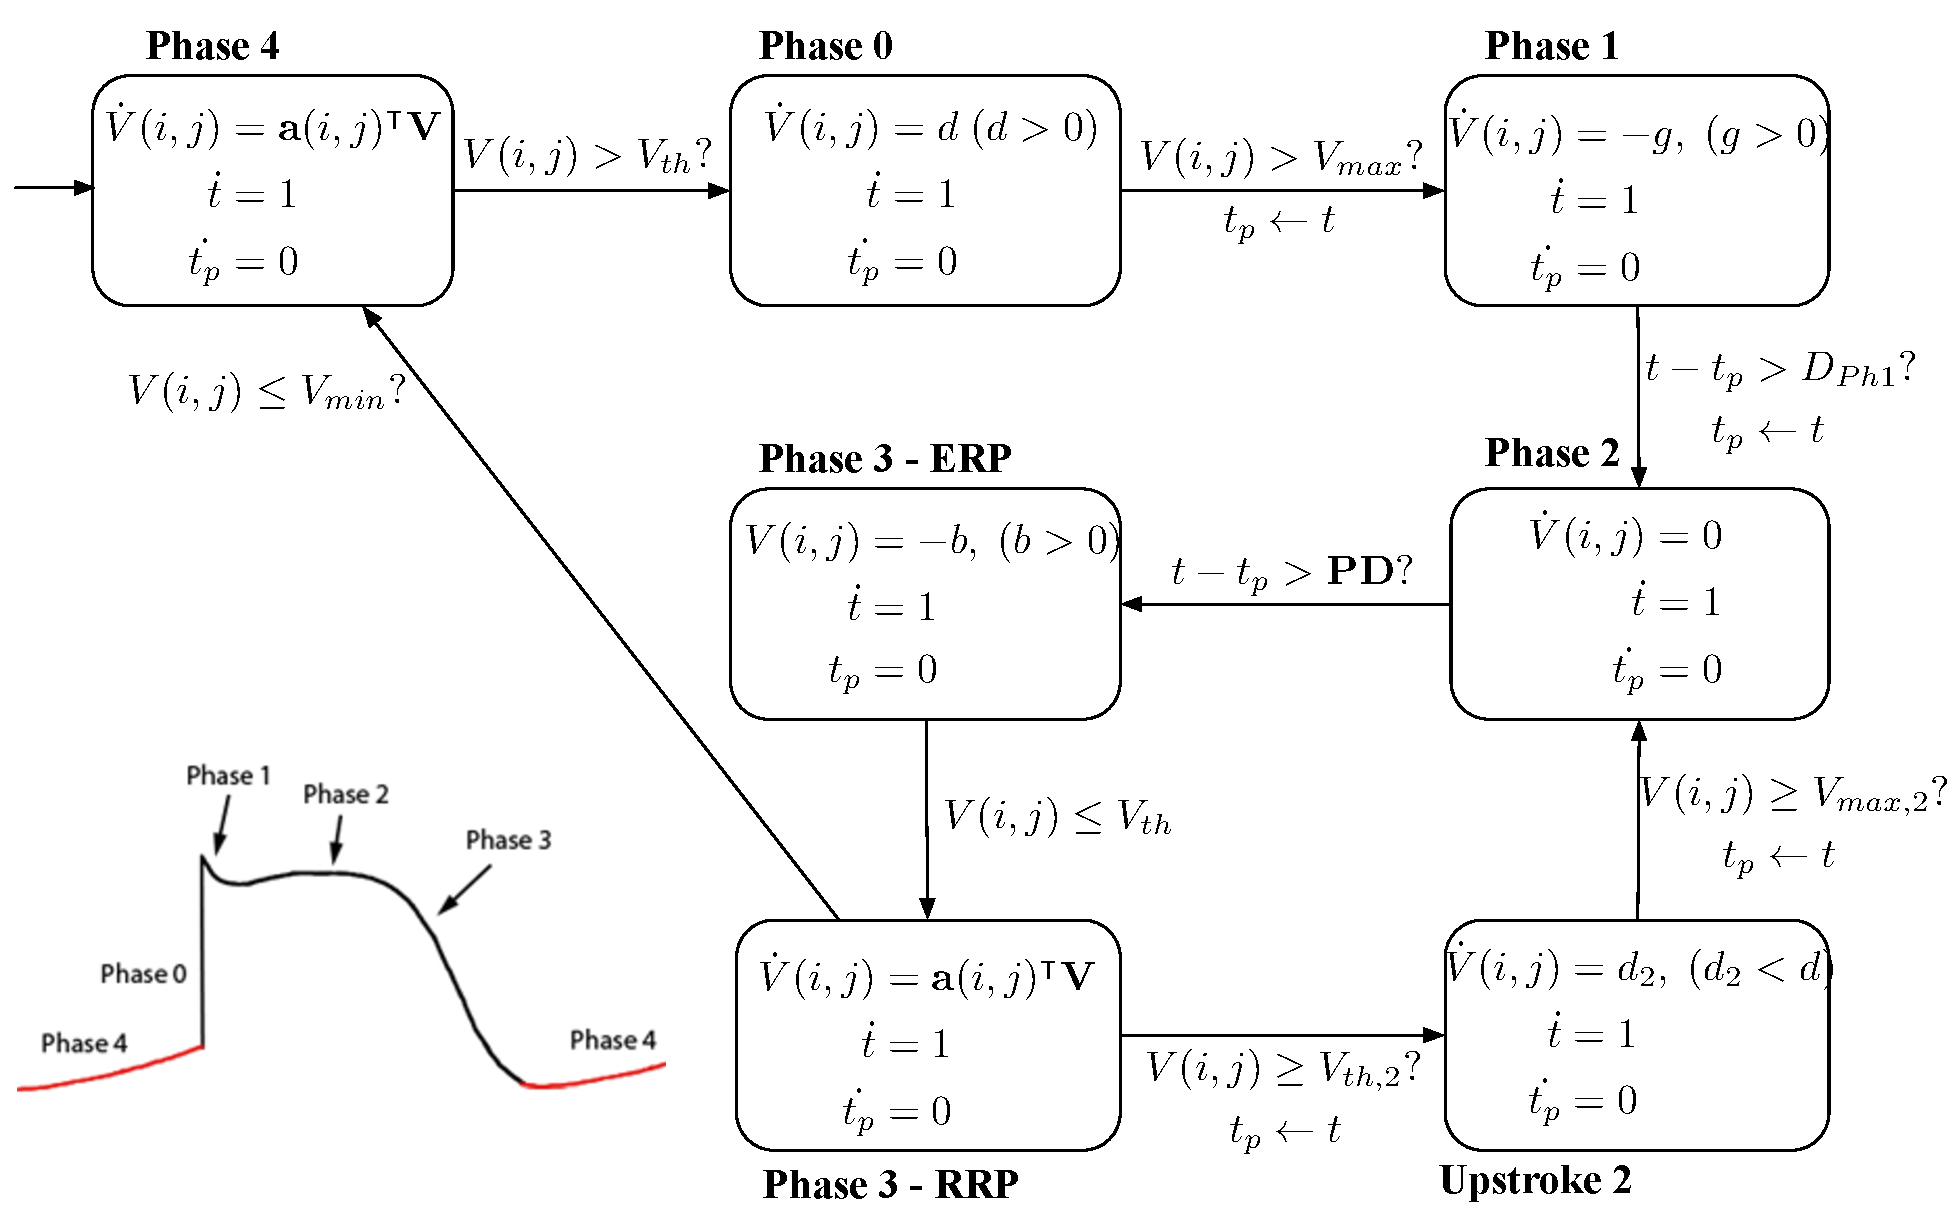
\includegraphics[scale=0.26]{figures/cellaut1v2}
	\vspace{-10pt}
	\caption{Hybrid model $\Sys_c$ of one cell of the heart model. AP figure from \cite{eplab}. 
		$V_{th,2}>V_{th}$, $V_{max,2}<V_{max}$}
	\vspace{-10pt}
	\label{fig:cellaut}
\end{figure}
%
The $(i,j)^{th}$ cell's voltage in Phase 4 depends on that of its neighbors and its own as follows \cite{Spector11_Emergence}
\begin{eqnarray}
\dot{V}(i,j,t) &=& \frac{1}{R_h}[V(i-1,j,t)+V(i+1,j,t) - 2V(i,j,t)] 
\nonumber \\ 
&& +  \frac{1}{R_v}[V(i,j-1,t) +  V(i,j+1,t) - 2V(i,j,t)]  
\nonumber\\
&=& a(i,j)^TV(t), \; a(i,j) \in \Re^{N^2}
\;
\end{eqnarray}
where $R_h$, $R_v$ are conduction constants that can vary across the myocardium.
Thus $V$ evolves according to a linear ODE $\dot{V} = AV$ where $A$ is the matrix whose rows are the $a(i,j)$. 
The two extra variables $t$ and $t_p$ are clocks.

\acp{ICD} observe the electrical activity through three channels (Fig.~\ref{fig:icd}).
Each signal is called an \ac{EGM} signal.
The signal read on a channel is the difference between two electrode potentials:
\begin{equation}
	\label{eq:vegm}
	\egm(t) = \frac{1}{K} \sum_{i,j} \left(\frac{1}{||(i,j)-p_0|| } - \frac{1}{||(i,j)-p_1||}\right) \dot{V}(i,j,t)
\end{equation}
where $p_0$ and $p_1$ are the electrodes positions.
This model was validated against real recordings taken in vitro \cite{StinnettDonnelly12_EGMresolution}.

\textbf{Extensions}. 
The APD restitution mechanism of heart cells, as modeled in \cite{Spector11_Emergence}, can be included in this model without changing its formal properties. 
%APD restitution models the dependence of the length of an \ac{AP} on the previous diastolic interval (roughly, the time between the end of one potential and the beginning of the next one).
%This is done in the online report.
%We used a simple constant slope for the variations of the \acp{AP}, as this was used in the original model \cite{Spector11_Emergence}. 
%Other more accurate shapes of the action potential are possible, while keeping the system STORMED.
%
%\subsection{Electrode measurement model}
%\label{sec:measurement}
%\acp{ICD} observes the electrical activity through three channels (Fig.~\ref{fig:icd}).
%Each signal is called an \ac{EGM} signal.
%The signal read on a channel is the difference between two potentials, and each potential may be modeled as being measured by an electrode located at position $p=(i_p,j_p)$ in the grid (Fig. \ref{fig:whole heart}).
%The potential measured by one electrode is given by \cite{StinnettDonnelly12_EGMresolution}:
%\begin{equation*}
%v_{E}(t) = \frac{1}{K} \sum_{i,j} \frac{I(i,j,t)}{||(i,j)-p||}
%\end{equation*}
%where $I(i,j,t)$ is the current density at $(i,j)$.
%In \cite{Spector11_Emergence} this current density is approximated as $I(i,j,t) \approx \dot{V}(i,j,t)$.
%%Thus we write 
%%\begin{equation}
%%\label{eq:apxI}
%%v_{E}(t) = \frac{1}{K} \sum_{i,j} \frac{\dot{V}(i,j,t)}{||(i,j)-p||}
%%\end{equation}
%We do not seek to verify the approximation - rather, we take it as our starting point.
%
%The \ac{EGM} signal is the difference of the two electrode potentials:
%\begin{equation}
%\label{eq:vegm}
%\egm(t) = \frac{1}{K} \sum_{i,j} \left(\frac{1}{||(i,j)-p_0|| } - \frac{1}{||(i,j)-p_1||}\right) \dot{V}(i,j,t)
%\end{equation}
%where $p_0$ and $p_1$ are the positions of the electrodes.
%This model was validated in vitro against real recordings taken by electrodes \cite{StinnettDonnelly12_EGMresolution}.

We now state and prove the main result of this section.
\begin{thm}
	Let $\Sys_{CA}$ be the whole heart cellular automaton model obtained by parallel composition of $N^2$ models $\Sys_c$ with state vector $x = [V, t,t_p,\egm ] \in \Re^{N^2}\times \Re^{3}$.
	Assume that all executions of the system have a duration of $D\geq 0$.
	Then $\Sys_{CA}$ is STORMED.
\end{thm}
\begin{prf}
	We verify each property of STORMED.
In this and all the proofs that follow, the approach is the same: $(ED)$ holds by Lemma \ref{prop:ED} because our state spaces are limited.
After establishing properties $(S), (T)$ and $(O)$, we draw up the constraints on $\phi$ and $\varepsilon$ imposed by reset and flow monotonicity (property (RM)). 
Then we argue that these constraints can be solved for $\phi$ and $\varepsilon$.
Often there is more than one solution and we just point to one.

\textbf{(S)} Separability holds because $V_{min} < V_{th}< V_{th,2} < V_{max,2} < V_{max}$ and $PD>0,D_{Ph_1}>0$. 
For example, on transition \textbf{Phase 4} $\rightarrow$ \textbf{Phase 0}, $V(i,j)=V_{th}$, which is separated from the next guard $\{V(i,j) > V_{max}\}$ by $|V_{max}-V_{th}|$.
%The only mode with two transitions is Phase 3 - RRP and its guards are $\{V(i,j) \leq V_{min}\}$ and $\{V(i,j) \geq V_{th,2}\}$ with separation $\sqrt{|V_{th,2}-V_{min}|}>0$.
\\
\textbf{(T)} All flows are linear or exponential and thus are TISG.
\\
\textbf{(O)} The flows, resets and guard sets are all definable in $\Lc_{\exp}$.
In particular the flow of $\dot{V} = AV$ is exponential with real exponent, and $\egm$ is a sum of exponentials and linear terms.
\\
\textbf{(RM)}
We seek a vector $\phi = (\phi_V,\phi_t,\phi_p,\phi_\egm)^T \in \Re^{N^2+3}$ such that resets and flows are monotonic along $\phi$.
Only transitions $p \rightarrow q \neq p$ are to be found in $\Sys_{CA}$, during which only $t_p$ is reset. 
Always, $t_p^+ = t \geq t_p^-$, thus the reset is indeed monotonic as can be seen by choosing any $\varepsilon >0$ and $\phi_p > \varepsilon$.

Monotonic flows: $\phi$ must also be such that in all modes:
\begin{equation*}
\phi \cdot (\theta_\ell(t+\tau;x) - \theta_\ell(t;x)) \geq \varepsilon ||\theta_\ell(t+\tau;x) - \theta_\ell(t;x)||
\end{equation*}
Decomposing, we want 
\begin{eqnarray*}
\label{eq:monotonic flow ca}
&&\phi_V \cdot(V(t+\tau) - V(t)) + \phi_t \tau + \phi_p \cdot 0 \\
&&\quad+ \phi_\egm \cdot (\egm(x,t+\tau) - \egm(x,t)) \geq \varepsilon ||\theta_\ell(x,t+\tau) - \theta_\ell(x,t)||
\end{eqnarray*}
Now note that all flows have bounded derivatives in every bounded duration of flow and are thus Lipschitz. 
Let $L_V$ be the Lipshitz constant of $V(t)$ and $L_{\egm}$ that of $\egm(t)$.
Then on the LHS of the above inequality we have 
$\phi_V \cdot(V(t+\tau) - V(t)) + \phi_\egm \cdot(\egm(t+\tau) - \egm(t)) \geq -\phi_V L_V \tau  -\phi_\egm L_{\egm} \tau$.
On the RHS we have  
$\varepsilon (L_V\tau + L_{\egm}\tau + \tau) \geq \varepsilon ( ||V(t+\tau) - V(t)|| + ||\egm(t+\tau) - \egm(t) ||  + \tau) \geq \varepsilon ( ||\theta_\ell(x,t+\tau) - \theta_\ell(x,t)||)$
Thus \eqref{eq:monotonic flow ca} is satisfied if the stronger inequality 
\[-\phi_V L_V \tau  -\phi_\egm L_{\egm} \tau + \phi_t \tau \geq \varepsilon (L_V\tau + L_{\egm}\tau + \tau) \]
is satisfied.
But this can be achieved by, for example, choosing $\phi_V = \phi_\egm = 0$ and $\phi_t \geq \varepsilon(L_V+L_{\egm}+1)$.
\\
\textbf{(ED)} Our system has bounded state spaces: $V$ and $\egm$ are voltages typically in the range $[-80,60]$ mV and $t_p \leq t \leq D$.
So (ED) holds by Lemma \ref{prop:ED}. 
\end{prf}